\section{Results}\label{sec:results}

\subsection{RL against SFT, and what a decode-time guard recovers}\label{sec:rlsft}
% [R1 R2 R3 R4 R5 R6 R13 D5; EVID tables 1-2; E01] GATE E-01
``SFT'' is the 385M SFT final; ``RL'' is the final general RL model (mixed-stage best); 214 rows flagged by the contamination audit are removed. RL improves \chrfpp{} on every benchmark (Table~\ref{tab:headline}); plain chrF over the 93 cells improves by $+8.59$ \ci{+8.43}{+8.76} and held-out AfriCOMET (76 cells) by $+0.0631$ \ci{+0.0620}{+0.0643}. All 54 FLORES+ and 24 NTREX languages improve on \chrfpp{}, chrF and AfriCOMET with intervals above zero; on MAFAND-MT 14 of 15 improve (pcm $-0.25$ \ci{-0.69}{+0.30}).

\begin{table}[t]
\centering\footnotesize\setlength{\tabcolsep}{2pt}
\caption{RL against SFT (language-macro \chrfpp{}, clean rows, 95\% paired bootstrap, one seed).}\label{tab:headline}
\begin{tabular}{@{}lrrl@{}}
\toprule
benchmark (n) & SFT & RL & RL $-$ SFT\\
\midrule
FLORES+ (54) & 22.85 & 31.66 & $+8.81$ \ci{+8.59}{+9.03}\\
NTREX (24) & 29.25 & 37.17 & $+7.91$ \ci{+7.69}{+8.12}\\
MAFAND-MT (15) & 35.77 & 40.78 & $+5.01$ \ci{+4.76}{+5.23}\\
all 93 cells & 26.59 & 34.55 & $+7.96$ \ci{+7.82}{+8.12}\\
\bottomrule
\end{tabular}
\end{table}

\textbf{Finishing and looping.} On FLORES+ (finished / loop / hypothesis-to-reference length) the SFT has 0.829 / 0.209 / 3.03, RL stage A 0.983 / 0.068 / 1.33 and the mixed best 0.995 / 0.048 / 1.14 (Appendix~\ref{app:rlsft}). Cutting the SFT's looping outputs at the loop onset, without changing the translation, lifts the SFT from 26.59 to 30.49 \chrfpp{}: \textbf{49\% of the gain is recovered by cutting loops}. 67 to 70\% of the gain sits in rows where either model failed, and about 41\% of the AfriCOMET gain is finishing. On rows where the SFT finished and did not loop, RL is still $+2.41$ \ci{+2.33}{+2.49} \chrfpp{} and $+0.0366$ AfriCOMET ahead, significant in 50 of 54 FLORES+ languages; the estimates favour different models and agree in sign and rough size.

\textbf{Decode-time loop guard (E-01).} Greedy decoding with a vLLM frequency penalty of 0.10 (best of a seven-setting dev grid; plain greedy 34.50, best 37.36 dev \chrfpp{}) gives SFT $26.59\to30.48$ and RL $34.55\to34.84$ \chrfpp{} over the 93 cells, and AfriCOMET (76 cells) SFT $0.565\to0.583$, RL $0.628\to0.631$ (Figure~\ref{fig:decomp}). \textbf{A guard on the SFT recovers the same 49\% of the \chrfpp{} gain (29\% of the AfriCOMET gain) without RL}; RL with the guard minus SFT with the guard is $+4.37$ \ci{+4.28}{+4.46} \chrfpp{} and $+0.0479$ \ci{+0.0469}{+0.0490} AfriCOMET ($+2.63$ \ci{+2.56}{+2.70} \chrfpp{} on rows where the guarded SFT is clean). Caveats: the optimum (0.10) lies at the edge of the grid, so the control may be under-tuned; a post-hoc dev-only extension was still rising (SFT dev \chrfpp{} 37.36 at 0.10, 37.97 at 0.20, 38.00 at 0.30, 38.25 at 0.50) and no full evaluation with a stronger penalty was run; one seed. With the guard, FLORES+ zgh and MAFAND-MT pcm are significantly worse for RL than for the SFT.

\begin{figure*}[t]
\centering
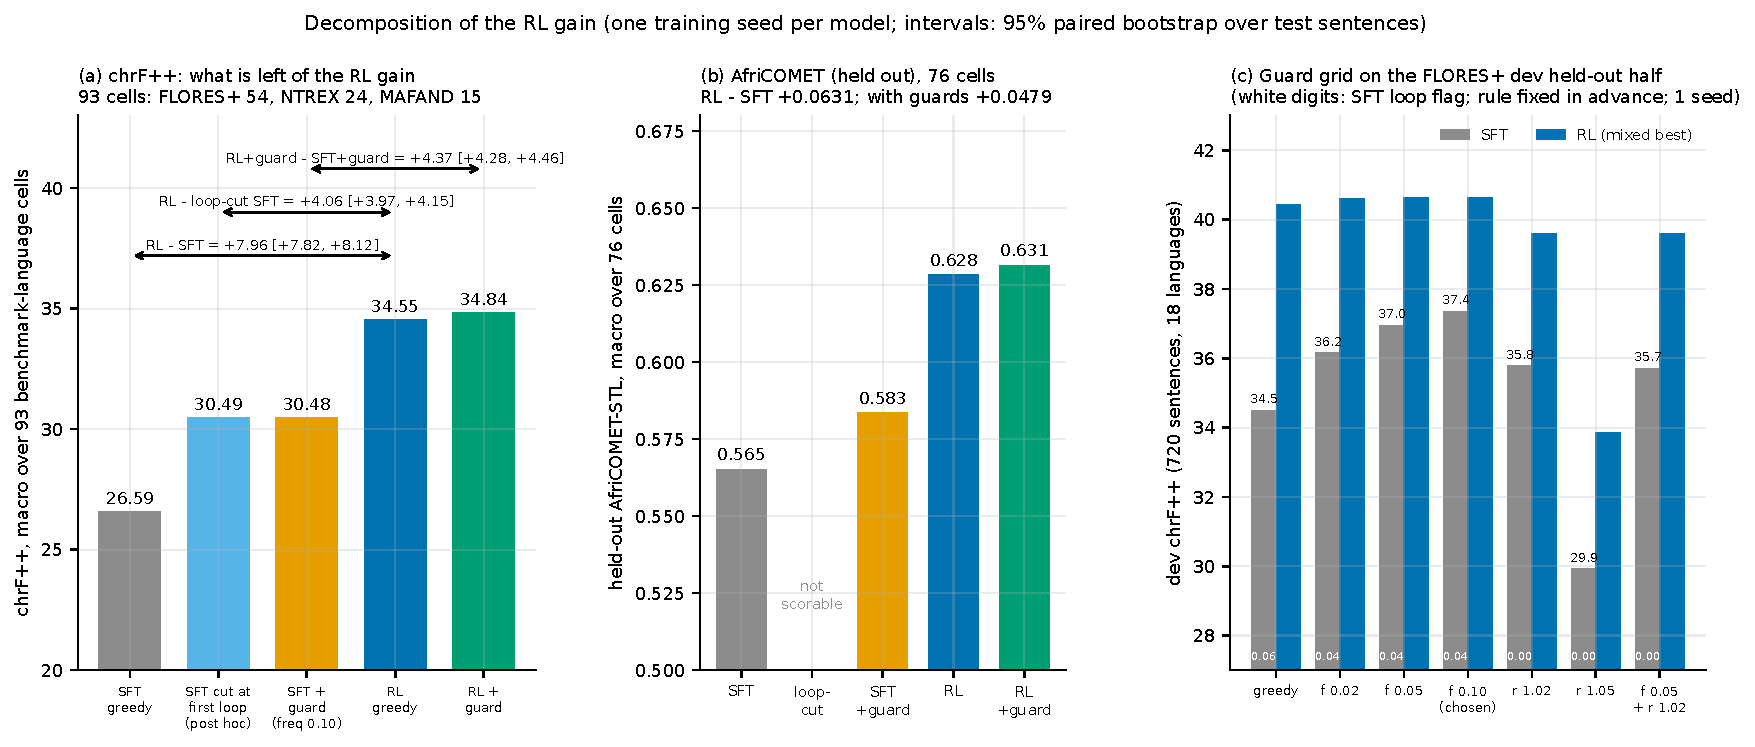
\includegraphics[width=\textwidth]{figures/fig3_decomposition_guard.pdf}
\caption{Decomposition of the RL gain with the decode-time guard (E-01). (a) Language-macro \chrfpp{} over 93 cells: SFT 26.59, SFT cut at its first loop 30.49 (post hoc), SFT with frequency penalty 0.10 30.48, RL 34.55, RL with guard 34.84; arrows give paired differences with 95\% CI. (b) Held-out AfriCOMET over 76 cells. (c) The seven-setting guard grid on the FLORES+ dev held-out half (720 sentences, 18 languages); the optimum (0.10) lies at the edge of the grid. One seed per model.}\label{fig:decomp}
\end{figure*}

\textbf{Growth and the earlier model.} The 385M SFT is significantly better than A0 on seven of eight benchmarks (FLORES+ $+5.31$ \ci{+5.13}{+5.50}, 46 languages; the comparison confounds depth with the extra stage-B SFT). In the same harness, on rows clean for both generations (E-13), it is behind our earlier 270M SFT on FLORES+ ($-2.35$ \ci{-3.25}{-1.38}), NTREX ($-4.13$) and MAFAND-MT ($-3.54$); after RL it is level on FLORES+ ($+0.35$ \ci{+0.08}{+0.62}) and NTREX ($+0.02$ \ci{-0.07}{+0.11}) and $1.55$ \chrfpp{} lower on MAFAND-MT, with data, steps, tokenizer layout and reward differing and only 4.7\% of FLORES+ rows kept (Appendix~\ref{app:sft}).

\subsection{Independent audit of the loop flag}\label{sec:degen}
% [R19-R24 DEGEN]
The reward's loop flag is the guard the RL was optimised against, so a missed loop type would be undercounted for RL. We re-measured with a detector sharing the idea but none of the code or constants (lzma-compressed size relative to human references of the same benchmark, language and length; repeated character 8-grams; repeated word 3-grams; each threshold set so that 0.1\% of 122,585 human references fire it). \textbf{The reward's flag is a lower bound:} on mixed-best FLORES+ the independent detector flags 1.77 \ci{1.71}{1.84} times as many outputs (0.0851 against 0.0480; SFT 0.3107 against 0.2095, ratio 1.48). The extra rows are finished partial repetitions: if they scored the average of their language's unflagged rows, mixed-best macro \chrfpp{} would rise by at most 0.19 (FLORES+), against 0.46 for the SFT, so the decomposition changes by 3.0\% to 4.4\% of the RL gains at most. Two further findings: 24.5\% of the 2,079 mixed-best rows above twice the reference length are flagged by neither detector, and \textbf{English output rises in the Arabic dialects and Tamazight} (aeb 0.215 to 0.449, ary 0.041 to 0.394, arz 0.006 to 0.098, zgh 0.001 to 0.049, SFT to mixed best; languages outside the RL prompt pool), so part of ``RL loops less'' there is a change from loops to English, while their \chrfpp{} stays at 2 to 9 (Appendix~\ref{app:degenapp}).

\begin{figure*}[t]
\centering
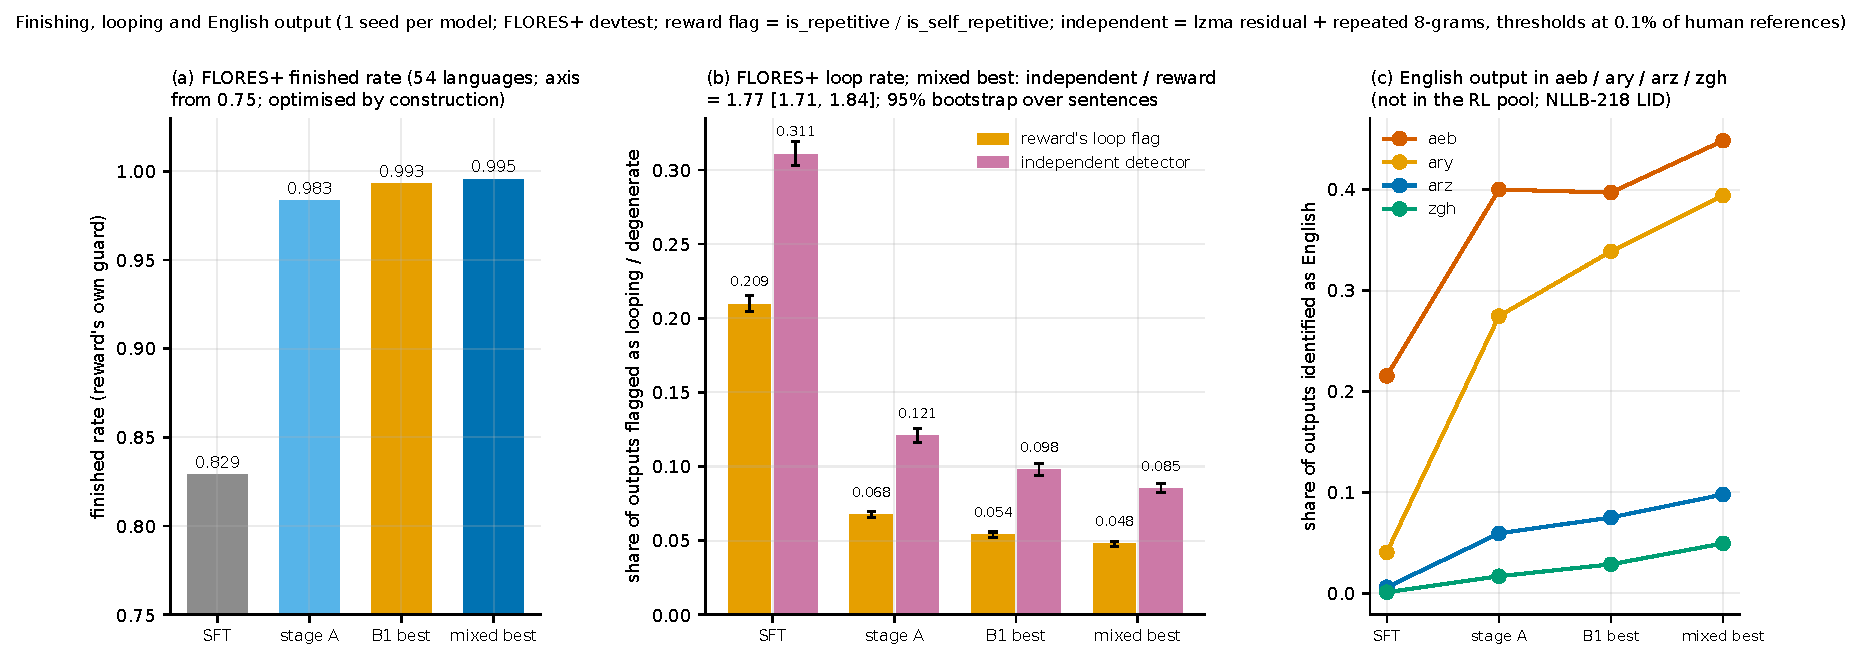
\includegraphics[width=\textwidth]{figures/fig7_loops_finishing.pdf}
\caption{Finishing, looping and English output on FLORES+ devtest (language macro, one seed per model). (a) Finished rate (54 languages; axis from 0.75). (b) Reward loop flag against the independent detector; error bars 95\% bootstrap over source sentences. (c) Share of outputs identified as English (NLLB-218 LID, $p\ge0.5$) in four languages outside the RL prompt pool.}\label{fig:loops}
\end{figure*}

\subsection{Where the gain accrues; seeds and ablations}\label{sec:seeds}
% [R8 E04 E11 M10 R17 R18]
Stage A gives 94\% of the SFT-to-B1 gain on FLORES+ (7.96 of 8.50); B1 adds $+0.54$ \ci{+0.49}{+0.59} and the mixed stage $+0.31$ \ci{+0.26}{+0.35} (NTREX $+0.30$, $+0.18$; MAFAND-MT nothing). B1 final (step 135) equals B1 best within noise. \textbf{Seeds (E-04).} Two extra runs of the stage-A recipe (100 steps, 20 languages, 49 cells) gain $+5.96$ \ci{+5.80}{+6.11} and $+5.90$ \ci{+5.74}{+6.05} \chrfpp{} over the SFT; they differ by \textbf{0.06} \ci{-0.02}{+0.14}. On those languages B1 best is $+0.17$ \ci{+0.12}{+0.21} over stage A, about three times the seed difference, while the mixed step is $+0.07$ \ci{+0.02}{+0.11}, the size of the seed difference: \textbf{we do not call the mixed step a gain}. This is one pair of seeds at step 100, not a seed study of later stages. RL aimed at eight weak West-African languages (85 steps, MBR guide) adds $+0.03$ \ci{-0.06}{+0.12} on its targets against a pre-registered $+1.0$ (negative result).

\textbf{Ablations (E-11).} One run per arm, 100 steps, forks of seed 2's step-40 state (Figure~\ref{fig:seeds}). Removing all four stage-A features costs \textbf{0.32} \ci{0.23}{0.41} \chrfpp{} (about 5\% of the gain, five times the seed difference); removing the reference domain costs 0.16 \ci{0.08}{0.25}; removing the beam guide costs 0.09 against seed 2 but $0.04$ \ci{-0.04}{+0.11} against seed 3, \textbf{not separable from seed noise}, for 25\% more step time. The KL rise is not caused by the features (median KL of steps 81 to 90: 0.116 without any feature, 0.120 to 0.123 in the other arms). The features are design choices with a small measured benefit.

\begin{figure*}[t]
\centering
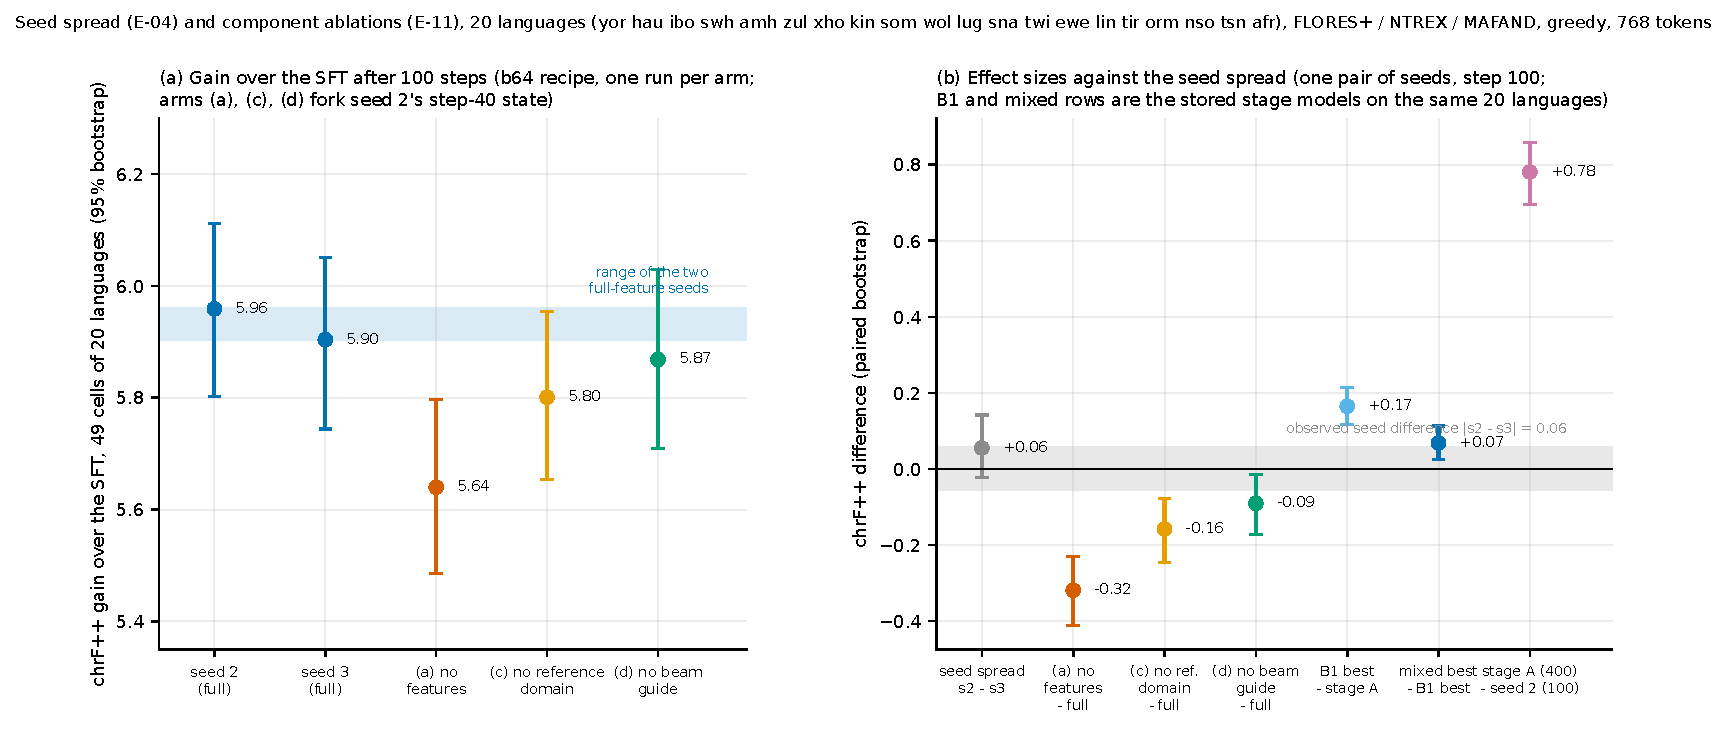
\includegraphics[width=\textwidth]{figures/fig16_e04_e11_seeds_ablations.pdf}
\caption{Seed spread (E-04) and ablation arms (E-11), 20 languages, 49 cells, greedy, 768 tokens, 95\% paired bootstrap. (a) \chrfpp{} gain over the SFT after 100 steps for two full-feature seeds and three ablation arms (shaded: range of the two seeds). (b) Effect sizes against the observed seed difference $|s_2-s_3|=0.06$: ablation arms minus seed 2, the B1 and mixed steps on the same languages, and the 400-step stage A minus seed 2. One pair of seeds, step 100.}\label{fig:seeds}
\end{figure*}

\subsection{Beam search and MBR (E-02)}\label{sec:decoding}
% [D1-D7 E02]
On 4,000 sentences (20 languages $\times$ 200 FLORES+ sentences) at 768 tokens, vLLM's beam search lets a runaway continuation beat every ended hypothesis, so the primary beam-4 (amended before any score) stops when 4 hypotheses have ended; a Hugging Face-style rule (\texttt{early\_stopping=False}) is a second beam. MBR-16 uses 16 samples plus the greedy output with \chrfpp{} as utility (metric-matched). Decoders help the SFT (beam-4 $+3.71$ \ci{+2.78}{+4.47}, MBR-16 $+5.96$ \ci{+5.37}{+6.49} \chrfpp{}); for the RL model MBR-16 adds $+0.92$ \ci{+0.81}{+1.03}, beam-4 (stop at 4) $-0.77$ \ci{-1.45}{-0.25} and the HF-rule beam $+0.83$ \ci{+0.67}{+1.00}: the sign of the RL beam result depends on the stopping rule. \textbf{Decoding does not replace RL}: RL greedy is $+1.60$ \ci{+1.34}{+1.88} \chrfpp{} ahead of the best decoded SFT (MBR-16, about 17 times the compute). RL minus SFT shrinks from $+7.56$ (greedy) to $+3.07$ (beam-4) and $+2.52$ (MBR-16): the RL gain is partly the same repair. Caveats: 20 languages, one checkpoint each; the beam numbers of an earlier 256-token study are not comparable (Appendix~\ref{app:decoding}). \textbf{Precision (E-09b):} bf16 and fp32 outputs differ between engines, but the SFT in fp32 on the full set scores $-0.04$ \ci{-0.13}{+0.07} \chrfpp{} against bf16 over the 93 cells, and the RL gain on FLORES+ is $+8.97$ \ci{+8.71}{+9.20} over the fp32 SFT against $+8.81$ over the bf16 SFT, so the bf16 harness does not overstate it; the RL model was not run in fp32.

\begin{table*}[t]
\centering\small\setlength{\tabcolsep}{3pt}
\caption{\chrfpp{} at 768 new tokens, language macro over 20 languages, 4,000 sentences per row, 95\% paired bootstrap (E-02).}\label{tab:e02}
\begin{tabular}{@{}lll@{}}
\toprule
decoding & SFT & RL (mixed best)\\
\midrule
greedy & 32.31 \ci{31.43}{33.38} & 39.87 \ci{39.17}{40.62}\\
beam-4, stop at 4 ended & 36.02 \ci{35.13}{36.95} & 39.10 \ci{38.20}{39.96}\\
beam-4, HF rule & 33.26 \ci{32.22}{34.46} & 40.70 \ci{40.00}{41.42}\\
MBR-16 & 38.27 \ci{37.60}{39.01} & 40.79 \ci{40.09}{41.54}\\
\bottomrule
\end{tabular}
\end{table*}

\subsection{Matched-compute continued-SFT control (E-03)}\label{sec:control}
% [R14 CTL7-CTL11] reports/e03_sft_control_2026-11-05.md; GATE E-03
To ask whether the GPU time of the RL chain (8.66 \GPUh{}) would do as well as more SFT, we continued the SFT final for 6,000 steps (8.4 h) at a constant learning rate of $10^{-5}$ (chosen by a probe fixed in advance), with 16 replay packs and 16 packs of TranslatePsy English-to-X pairs \citep{gritta2026translatepsy} per step: NLLB-3.3B translations of MADLAD-400 sentences for 19 languages, 277,900 pairs each, scanned against the protected index and used once. The decision rule, primary endpoint (language-macro \chrfpp{} over 93 cells, RL minus control) and language panels were written down before any benchmark of the control was looked at. \textbf{Only the 6,000-step checkpoint was evaluated}; the stage-A-matched (3,100) and mixed-best-matched (4,800) checkpoints exist but were not evaluated.

\begin{table}[t]
\centering\footnotesize\setlength{\tabcolsep}{3pt}
\caption{Continued-SFT control against the RL mixed best; language-macro \chrfpp{}, clean rows, 95\% paired bootstrap; TP = the 19 TranslatePsy languages. Held-out AfriCOMET, RL $-$ control: $+0.0183$ (all), $-0.0249$ (TP), $+0.0883$ (other).}\label{tab:e03}
\begin{tabular}{@{}lccl@{}}
\toprule
cells & control & RL & RL $-$ control\\
\midrule
all (93) & 29.97 & 34.55 & $+4.58$ \ci{+4.45}{+4.70}\\
TP (47) & 41.37 & 41.34 & $-0.03$ \ci{-0.13}{+0.09}\\
other (46) & 18.32 & 27.61 & $+9.29$ \ci{+9.09}{+9.49}\\
\bottomrule
\end{tabular}
\end{table}

The registered rule had four conditions: lower bound of the overall difference above $+1.0$ (met: $+4.58$ \ci{+4.45}{+4.70}), AfriCOMET lower bound above 0 (met: $+0.0183$ \ci{+0.0172}{+0.0192}), difference above 0 on the other languages (met) and difference above 0 on the 19 TranslatePsy languages (\textbf{not met}: $-0.03$). \textbf{By the rule as registered the verdict is ``inconclusive''}, and we did not change the rule. Reading the panels: where a teacher-translated corpus exists, continued SFT matches RL in \chrfpp{}, largely fixes finishing and looping (FLORES+ finished 0.993 against 1.000 for RL), and is ahead on the neural metrics; on the other languages it changes almost nothing ($+0.15$ \chrfpp{} over the SFT on FLORES+, \ci{-0.03}{+0.32}), while RL improves them all from its own samples ($+9.29$). The overall endpoint alone reads ``RL is better'', the 19 languages alone ``comparable''; neither is the registered verdict. Caveats: one seed, one learning rate, one budget point; the control is not information-matched (NLLB-3.3B scores 38.80 against 26.30 for the SFT on 43 languages), and the TranslatePsy rows were filtered with AfriCOMET, SSA-COMET and MetricX, so those neural metrics favour the control; chrF and \chrfpp{} are the evidence.

\begin{figure*}[t]
\centering
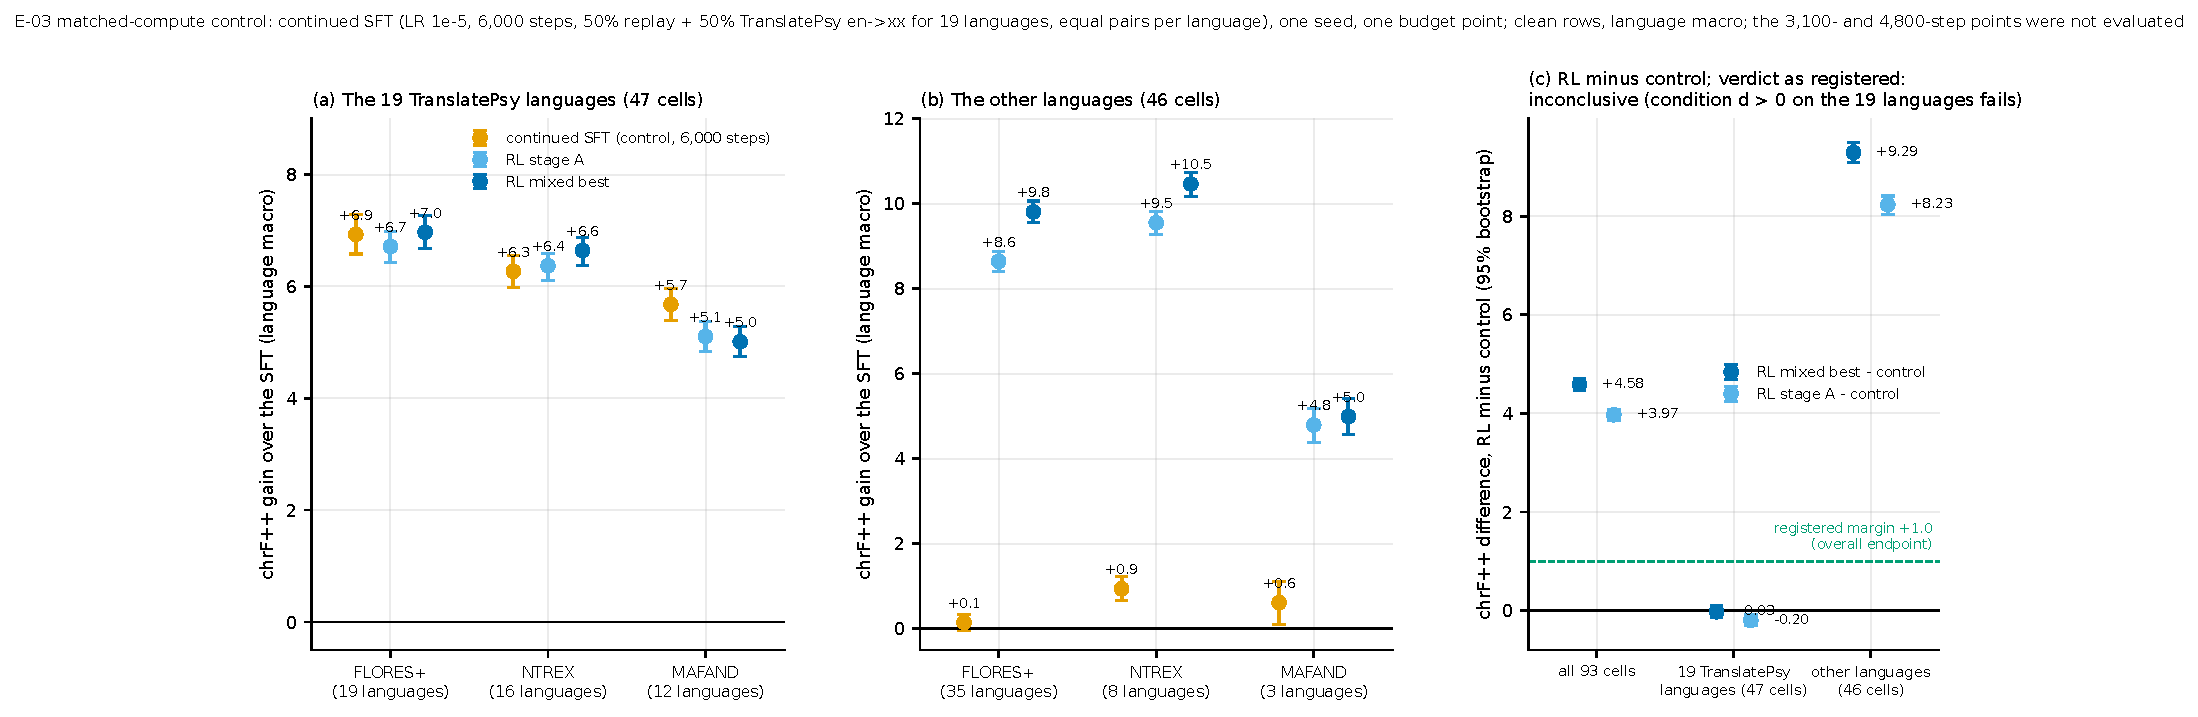
\includegraphics[width=\textwidth]{figures/fig14_e03_control.pdf}
\caption{Matched-compute continued-SFT control (E-03). (a, b) \chrfpp{} gain over the SFT (language macro, 95\% bootstrap) of the control, RL stage A and RL mixed best by benchmark, for the 47 cells of the 19 TranslatePsy languages (a) and the 46 other cells (b). (c) RL minus control for all 93 cells and for the two panels, with the registered $+1.0$ margin; the registered verdict is inconclusive. One seed per model; only the 6,000-step checkpoint was evaluated.}\label{fig:e03}
\end{figure*}

\subsection{Comparison with NLLB-200}\label{sec:nllb}
% [N1-N6 NLLBRL]
NLLB-200 3.3B (the 3.3B variant of its model card) has about 8.6 times the parameters of our 385M model. On the 43 languages shared with the published FLORES-200 devtest table, the mixed best reaches 35.54 \chrfpp{} against 38.80 for NLLB-3.3B ($-3.26$, language-bootstrap \ci{-4.29}{-2.20}; 92\%; SFT 26.30, $-12.50$, 68\%): RL closes 74\% of the gap, and the remaining gap is not a finishing artefact (the mixed best finishes at least 0.99 in every language). It matches or beats NLLB-3.3B on 7 of 43 languages, all in the lowest tertile (e.g. yor $+5.43$, fon $+2.95$); the largest gaps are amh $-11.28$, kin $-9.74$, kea $-8.72$. Caveats: FLORES-200 against FLORES+ references, NLLB beam against our greedy (beam and MBR move our \chrfpp{} by $-0.77$ to $+0.92$), the 11 hardest languages have no NLLB row, five of the 43 languages had an NLLB pseudo-reference reward term, the yor value is anomalously low, intervals are over languages, one seed. We state only that, size-aware, the model reaches 92\% of NLLB-3.3B's \chrfpp{} on these languages and matches or beats it on 7 of 43; we do not claim to beat NLLB or to be competitive with it overall.

\begin{figure*}[t]
\centering
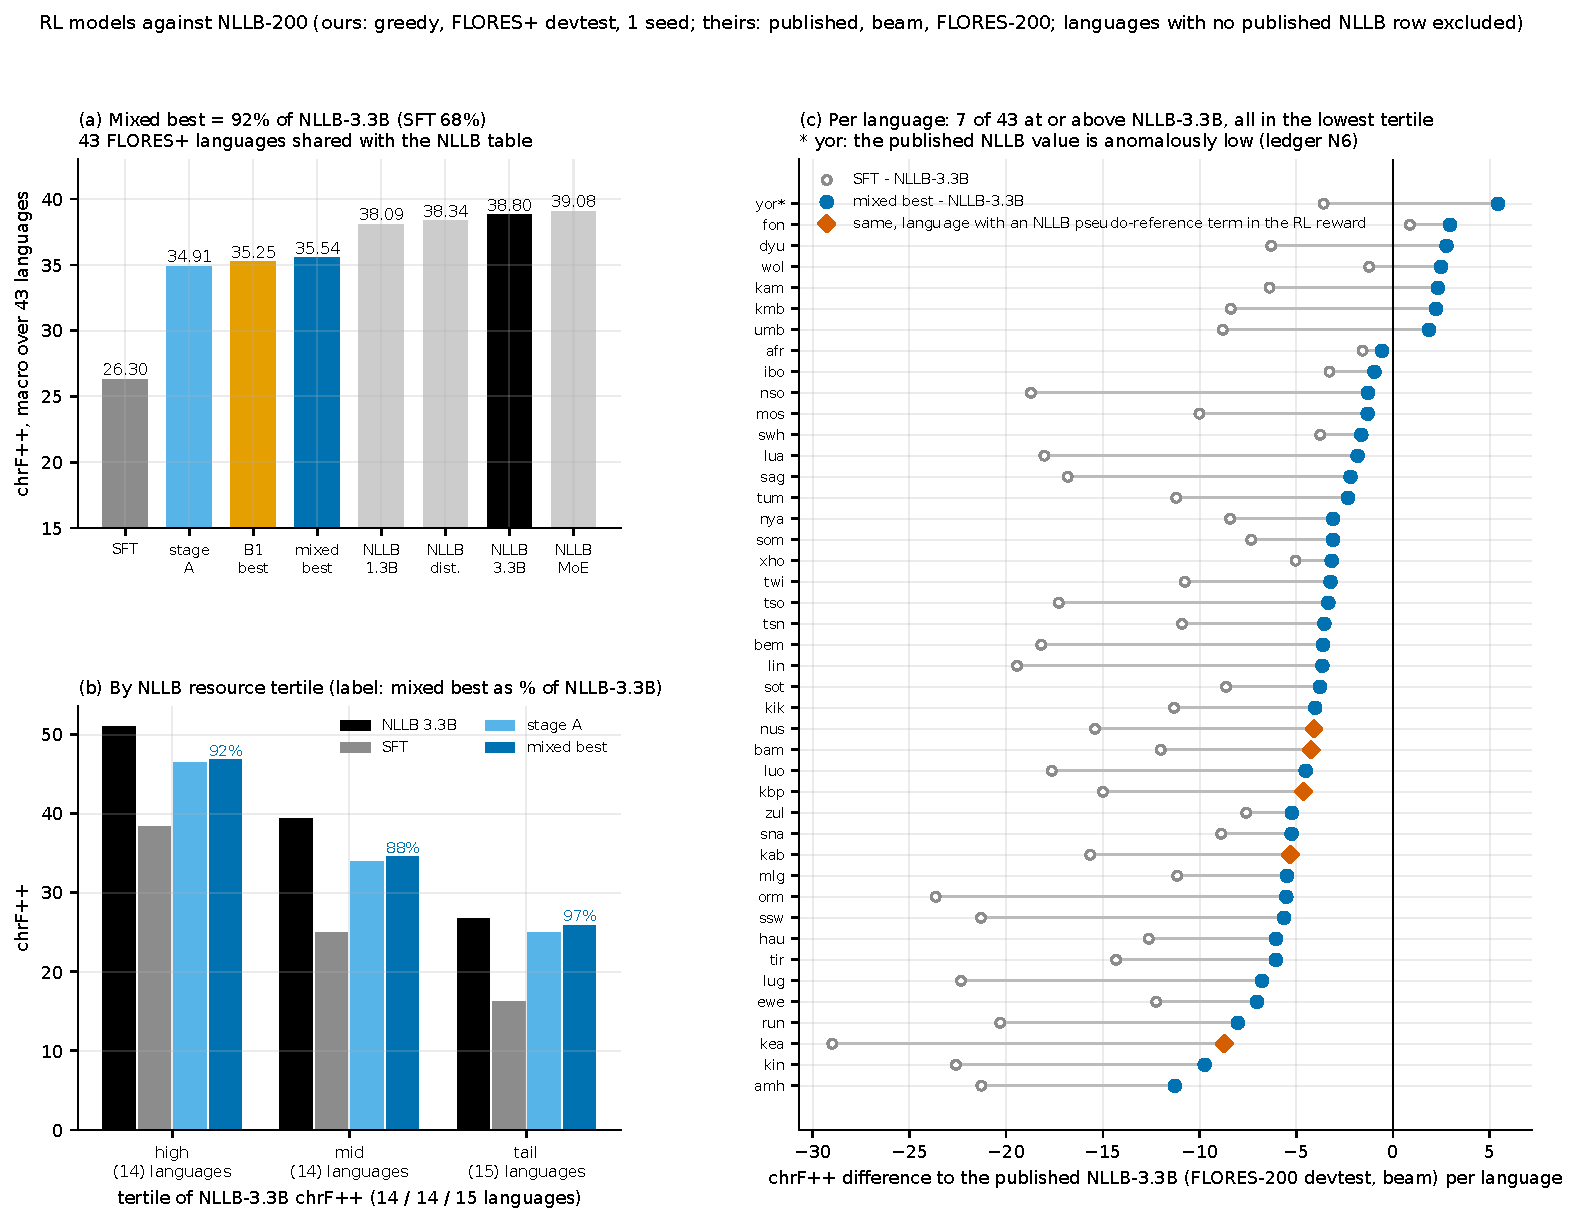
\includegraphics[width=0.62\textwidth]{figures/fig4_nllb_43.pdf}
\caption{RL models against NLLB-200 on the 43 shared FLORES+ languages (ours: greedy, one seed per model; NLLB: published FLORES-200 devtest, beam). (a) Language-macro \chrfpp{}: mixed best 35.54 against NLLB-3.3B 38.80 (92\%; SFT 68\%). (b) By tertile of NLLB-3.3B \chrfpp{} (14/14/15 languages). (c) Per-language difference to NLLB-3.3B, SFT (open) and mixed best (filled); orange diamonds: languages with an NLLB-3.3B pseudo-reference reward term; yor$^*$: anomalously low published value. Intervals are over languages only.}\label{fig:nllb}
\end{figure*}

\subsection{Science and long-document RL}\label{sec:science}
% [SC1-SC6 DL1-DL5 P4 E05 E15 E16]
A science SFT with weight interpolation ($\alpha=0.5$) gives surface gains on AfriScience-MT (chrF $+1.2$) and no SSA-COMET-QE gain (0.6130 to 0.6118). A science RL adds $+0.46$ chrF \ci{+0.27}{+0.65} and $+0.0053$ AfriCOMET on test sentences over its start, and nothing at document level. \textbf{The science SFT, not the science RL, carries the science gain (E-14):} the same RL started from the mixed best, without the science SFT, ends $-1.44$ chrF \ci{-1.61}{-1.25} and $-0.0082$ AfriCOMET \ci{-0.0101}{-0.0065} below the executed science RL and adds only $+0.26$ chrF \ci{+0.12}{+0.39} over its start, so by the registered rule the science SFT is needed; SSA-COMET-QE rates it level ($-0.0006$ \ci{-0.0018}{+0.0007}), a reward-family effect rather than evidence of quality. One seed, one out-of-memory restart, final checkpoint only (Appendix~\ref{app:docs}). Whole-document generation (4,096 tokens) fails for the 385M models; a long-document RL raises whole-document finishing from 0.70 to 0.82 ($+0.125$ \ci{+0.046}{+0.204}) and lowers the loop rate from 0.85 to 0.73, but 72 to 73\% of documents still loop and chunked decoding is required; the earlier 270M model is as good or better at document level. Table~\ref{tab:sci} gives sentence-level scores for every stage (SSA-COMET-QE is of the reward family; the first RL stage adds $+0.043$ and later stages at most $+0.005$ more, while chrF and AfriCOMET keep rising slightly).

\begin{table}[t]
\centering\footnotesize\setlength{\tabcolsep}{3pt}
\caption{AfriScience-MT test, sentence level (970 sentences per language; macro over amh hau lug nso yor zul; greedy; one seed per stage). SSA-QE = SSA-COMET-QE, of the reward family for every RL row.}\label{tab:sci}
\begin{tabular}{@{}lccc@{}}
\toprule
stage & chrF & AfriCOMET & SSA-QE\\
\midrule
SFT & 36.00 & 0.6064 & 0.5686\\
RL stage A & 45.06 & 0.6822 & 0.6118\\
RL mixed best & 45.40 & 0.6828 & 0.6130\\
science RL w/o SFT (E-14) & 45.66 & 0.6850 & 0.6153\\
science SFT ($\alpha=0.5$) & 46.63 & 0.6879 & 0.6118\\
science RL final & 47.10 & 0.6932 & 0.6158\\
long-document RL final & 47.16 & 0.6936 & 0.6165\\
\bottomrule
\end{tabular}
\end{table}
